\documentclass[10pt]{article}
\usepackage{sectsty}
\usepackage{graphicx}
\usepackage{tabu}
\subsectionfont{\small}


\newcommand{\reqinit}{
	% Create a new counter for keeping track of the last number
	\newcounter{reqcountbackup}
	% Create a new counter for the custom label
	\newcounter{reqcount}
	% Redefine the command for the last counter so when it is calledcs
	% it prints the number like this in a bold font: R<number>
	\renewcommand{\thereqcount}{\textbf{R\arabic{reqcount}}}
}

% Used to define the start of the requirements
\newcommand{\reqstart}{
	% Indicate the start of a new list and tell it to use the redefined
	% command and corresponding counter for every item
	\begin{list}{\thereqcount}{\usecounter{reqcount}}
		% Important part: set the value of the used counter to the
		% same value of the backup counter.
		\setcounter{reqcount}{\value{reqcountbackup}}
	}
	
	% Used to define the end of the requirements
	\newcommand{\reqend}{
		\setcounter{reqcountbackup}{\value{reqcount}}
		% Mark the end of the list environment
	\end{list}
}

\begin{document}
	
	\begin{titlepage}
		\centering
		\vspace*{\fill}
		
		\vspace*{0.5cm}
		
		\huge\bfseries
		\rule{\textwidth}{1.6pt}\\[\baselineskip]
		AI Auto Car Classifier \\Testing Policy
		
		\vspace*{0.5cm}
		
		\large Edited by: \\[\baselineskip]
		
		{Fiwa Lekhuleni\\Abhinav Thakur\\Vincent Soweto\\Andrew Jordaan\\Keorapetse Shiko}
		
		\rule{\textwidth}{1.6pt}\\[\baselineskip]
		
		
		\vspace*{\fill}
	\end{titlepage}
	
	\newpage
	
	\tableofcontents
	
	
	\newpage
	
\section{Introduction}

\hspace{5cm}

This document provides information on the various testing mechanisms that are implemented in the system. It specifies the technologies and the policy to be followed in terms of the testing. A testing policy provides a defined structure that encourages transparency and effective team work. 

\hspace{5cm}


\section{Testing Objectives}

\hspace{5cm}

Through testing, the aim is to investigate how the system is executing the certain tasks. The testing objectives are to define a structure of testing each subsystem and to see how the subsystems interact with each other, facilitate consistent and continuous testing, early detection of defects and to decrease the complexity of debugging.

\newpage
\section{Types of Tests}

\hspace{5cm}

Conventional black-box testing is used by functional testing.
Software testing is a dynamic validation activity to detect defects and undesirable behaviour in the software being tested, and demonstrated that the software satisfies its requirements and constraints.

\hspace{5cm}


\subsection{Unit Testing}

 Unit testing entails separating each individual component (unit) of the system and testing them individually to ensure that they all behave in the expected manner, in line with the specified requirements. The Mocha framework is used to conduct the unit tests.


\hspace{5cm}

 \subsection{Automated Testing and Continuous Integration}
 Travis CI is the tool chosen for our continuous integration. 
It executes automated testing by running the unit tests after each commit.
Travis CI displays the test results and maintains logs for each test executed.
 
  \newpage
 \section{Testing Methods and Techniques}
 
 \subsection{Test Cases}
 \hspace{5cm}
 


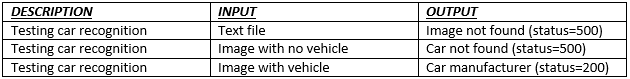
\includegraphics[width=15cm,height=2cm]{table.png}
\caption{Functional Testing}
    
\hspace{5cm}
 
 
The test scripts will have the “*.test.js” extension and will be stored under the “test” folder. The "npm test" command runs the Mocha test scripts and displays the test results on the terminal.

\newpage
An example of a test is given below:

\hspace{5cm}

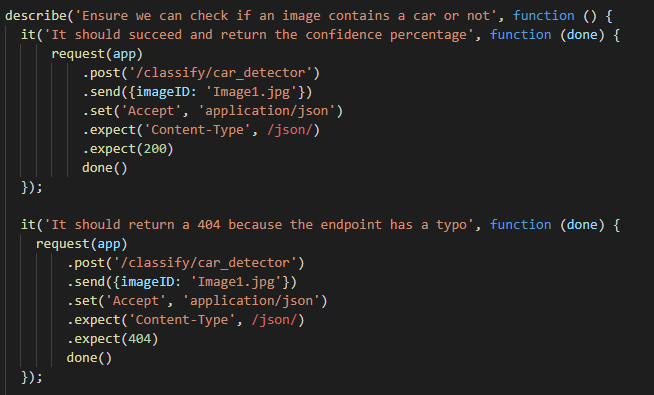
\includegraphics[width=15cm,height=12cm]{unit.png}
\caption{Unit Test}
    

 \newpage


\section{Test Coverage}
\hspace{5cm}

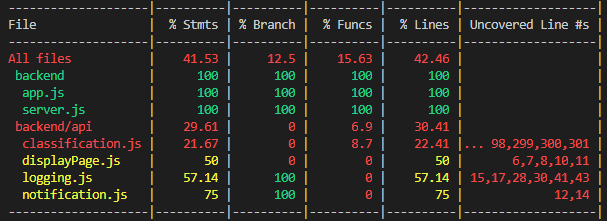
\includegraphics[width=15cm,height=9cm]{cover.png}
\caption{Test Coverage}

\newpage

\section{Required Resources}

\hspace{5cm}

A few resources are required to conduct the tests. Since the system is a Node application, "npm" is required to call the test command.
The Mocha framework executes the unit tests, this can be done in less than a minute.
Travis CI can be found on it's website, it runs the tests and deployment in less than 5 minutes.


 \end{document}